\documentclass{article}
\usepackage{lipsum}
\usepackage{enumerate}
\usepackage{amsmath, amssymb, amsthm, amsfonts}
\usepackage{url}
\usepackage{fullpage}
\usepackage{graphicx}
\usepackage[backref, colorlinks=true, linkcolor=blue, citecolor=green, urlcolor=blue]{hyperref}


\newtheorem{theorem}{Theorem}
\newtheorem{lemma}{Lemma}
\newtheorem{corollary}{Corollary}
\newtheorem{definition}{Definition}
\newtheorem{proposition}{Proposition}
\newtheorem{procedure}{Procedure}
\newtheorem{construction}{Construction}
\newtheorem{example}{Example}
\newtheorem{remark}{Remark}
\newtheorem{claim}{Claim}

\newcommand{\Rea}{{\mathbb R}}
\newcommand{\Int}{{\mathbb Z}}
\newcommand{\Rat}{{\mathbb Q}}
\newcommand{\Cmp}{{\mathbb C}}
\newcommand{\Nat}{{\mathbb N}}

\setlength{\oddsidemargin}{.25in}
\setlength{\evensidemargin}{.25in}
\setlength{\textwidth}{6.25in}
\setlength{\topmargin}{-0.0in}
\setlength{\textheight}{8.9in}

% this is for proof environment
\renewenvironment{proof}{\noindent{\bf Proof:} \hspace*{1mm}}{
	\hspace*{\fill} $\Box$ }
\newenvironment{proof_of}[1]{\noindent {\bf Proof of #1:}
	\hspace*{1mm}}{\hspace*{\fill} $\Box$ }
\newenvironment{proof_claim}{\begin{quotation} \noindent}{
	\hspace*{\fill} $\diamond$ \end{quotation}}


\renewcommand{\thefootnote}{\fnsymbol{footnote}} %将脚注符号设置为fnsymbol类型,即特殊符号表示

\title{
   \textbf{Overview: A Little Charity Guarantees Almost Envy-Freeness } \\ 
   \large Algorithmic Game Theory, 2023 Spring\footnotemark[1]
}

\author{Linkang Dong\footnotemark[2]}
\date{\today}



\begin{document}

% title
\maketitle
\footnotetext[1]{This is the final project of Algorithmic Game Theory, 2023 Spring, instructed by Prof. Zhengyang Liu.}
\footnotetext[2]{Department of Computer Science, Beijing Institute of Technology, China.
Email: donglinkang@bit.edu.cn, Student ID: 1120212477, Phone Num: +86 17876964909. Please contact me if any question in your convenience. }

% abstract
\begin{abstract}

    Envy-freeness is a widely explored concept of fairness, but it does not always exist in the context of indivisible goods. An alternative notion of fairness that we consider is “envy-freeness up to any good” (EFX). Under EFX, no agent envies another agent after any single good is removed from the latter's bundle. The existence of such an allocation is currently unknown.
    
    This study\cite{chaudhury2020little} demonstrates the existence of a partition of the goods into $n+1$ subsets, denoted as $(X_1, \ldots, X_n, P)$, where $X_i$ represents the bundle allocated to agent $i$, and the set $P$ remains unallocated or is donated to charity. The proposed allocation satisfies the following conditions:
    
    \begin{enumerate}
        \item Envy-freeness up to any good,
        \item No agent values $P$ higher than their own bundle,
        \item The number of goods allocated to charity is fewer than $n$, i.e., $|P| < n$ (typically $m \geq n$).
    \end{enumerate}
    
    The proof leads to a pseudo-polynomial time algorithm to find such an allocation. This algorithm extends its applicability to cases where agents have general valuation functions, not limited to just gross-substitute valuations. Furthermore, when $|P|$ is large, i.e., close to $n$, the proposed allocation also guarantees a good maximin share (MMS). Additionally, a minor variant of the algorithm establishes the existence of an allocation that achieves at least a $\frac{4}{7}$ groupwise maximin share (GMMS), which is a stronger notion of fairness than MMS. This improvement supersedes the current best approximate GMMS allocation bound of $\frac{1}{2}$. The findings in this paper go beyond the preliminary version published in SODA 2020~\cite{doi:10.1137/20M1359134} \footnotemark[3]

\end{abstract}

\footnotetext[3]{{We will not cover this part in this report, and it is enough to know that the two key contributions: the pseudo-polynomial algorithm accommodates agents with general valuation functions, and a relaxed definition of the “most envious agent” is introduced, which adds to the practicality and applicability of the proposed allocation.}}


% contents
\newpage
\tableofcontents



% body
\newpage
\section{Introduction} \label{sec:intro}
In this report, the final project of Algorithmic Game Theory, 2023 Spring, we present an overview of the paper A Little Charity Guarantees Almost Envy-Freeness \cite{chaudhury2020little}. We first introduce the architecture and give a brief introduction \ref{sec:intro} of the paper, focussing on which problem it tries to solve. Then, we will introduce the preliminaries \ref{sec:pre} of the paper, including the definition of the problem, solution, and the algorithm. After that, we will introduce the core ideas \ref{sec:core} of the paper.\footnote{However, we haven't give the proof part for the core ideas, since it is too long and complex. If you are interested in it, please refer to the original paper \cite{chaudhury2020little}.} Finally, we conclude the overview of the paper and give some acknowledgements \ref{sec:ack}.

\section{Preliminaries} \label{sec:pre}
Fair division of indivisible goods is a well-studied problem in which the objective is to distribute $m$ goods to $n$ agents in a manner that is considered “fair”. Each agent has a valuation for every subset of goods, and the challenge arises due to the indivisibility of the goods.

\subsection{Envy-freeness}

An allocation is a partition of $M$ into disjoint subsets $X_1, \ldots, X_n$ where $X_i$ is the set of goods given to agent $i$. 
Assume that each agent $i$ has a valuation function $v_i: 2^M \rightarrow \mathbb{R}$, where $v_i(X_i)$ is the value of $X_i$ to agent $i$.

One of the most well-studied notions of fairness(an allocation can be considered “fair”) is Envy-freeness. Every agent has a value associated with each subset of $M$, and agent $i$ envies agent $j$ if $i$ values $X_j$ more than $X_i$. Obviously, an allocation is envy-free if no agent envies another agent, and we can define it formally as follows:

\[
    \forall i, j \in [n], v_i(X_i) \geq v_i(X_j)  
\]

Someone also defines envy-freeness as follows:

\[
  \text{For each agent i}, v_i(X_i) \geq v_i(X_j), \forall j \in [n] 
\]

An envy-free allocation can be regarded as a fair and desirable partition of $M$ among the $n$ agents since no agent envies another \cite{DBLP:journals/corr/PlautR17}.

\subsection{Relaxation of Envy-freeness}

An envy-free allocation of the given set of goods need not exist because of the indivisibility of the goods.
Consider the following simple example with two agents and a single good that both agents desire: one of the agents has to receive this good, and the other agent envies her. Since envy-free allocations need not exist, several relaxations have been considered.

\subsubsection*{Envy-freeness up to one good (EF1)}

In an EF1 allocation, agent $i$ may envy agent $j$, however this envy would vanish as soon as some good is removed from $X_j$.\footnote{Note that no good is really removed from $X_j$: just a way of assessing how much $i$ values $X_j$ more than $X_i$. That is, if $i$ values $X_j$ more than $X_i$, then there exists some $g \in X_j$ such that $i$ values $X_i$ at least as much as $X_j \setminus \{g\}$. Going back to the example of two agents and a single good, the allocation where one agent receives this good is EF1.}

An allocation is envy-free up to one good if there is at most one good that an agent envies another agent for. Formally, an allocation is envy-free up to one good if there exists at most one pair of agents $i, j \in [n]$ such that $v_i(X_i) < v_i(X_j)$.

\subsubsection*{Envy-freeness up to any good (EFX)}

An allocation is envy-free up to any good if there is no good that an agent envies another agent for. Formally, an allocation is envy-free up to any good if for every pair of agents $i, j \in [n]$, $v_i(X_i) \geq v_i(X_j)$.

 It is known that EF1 allocations always exist; as shown by Lipton et al.~\cite{10.1145/988772.988792}, such an allocation can be efficiently computed.

Caragiannis et al.~\cite{10.1145/3355902} introduced a notion of envy-freeness called EFX that is stronger than EF1. An EFX allocation is one that is “envy-free up to any good”. In an EFX allocation, agent $i$ may envy agent $j$, however this envy would vanish as soon as any good is removed from $X_j$. Thus every EFX allocation is also EF1 but not every EF1 allocation is EFX.

\begin{figure}[htbp]
    \centering
    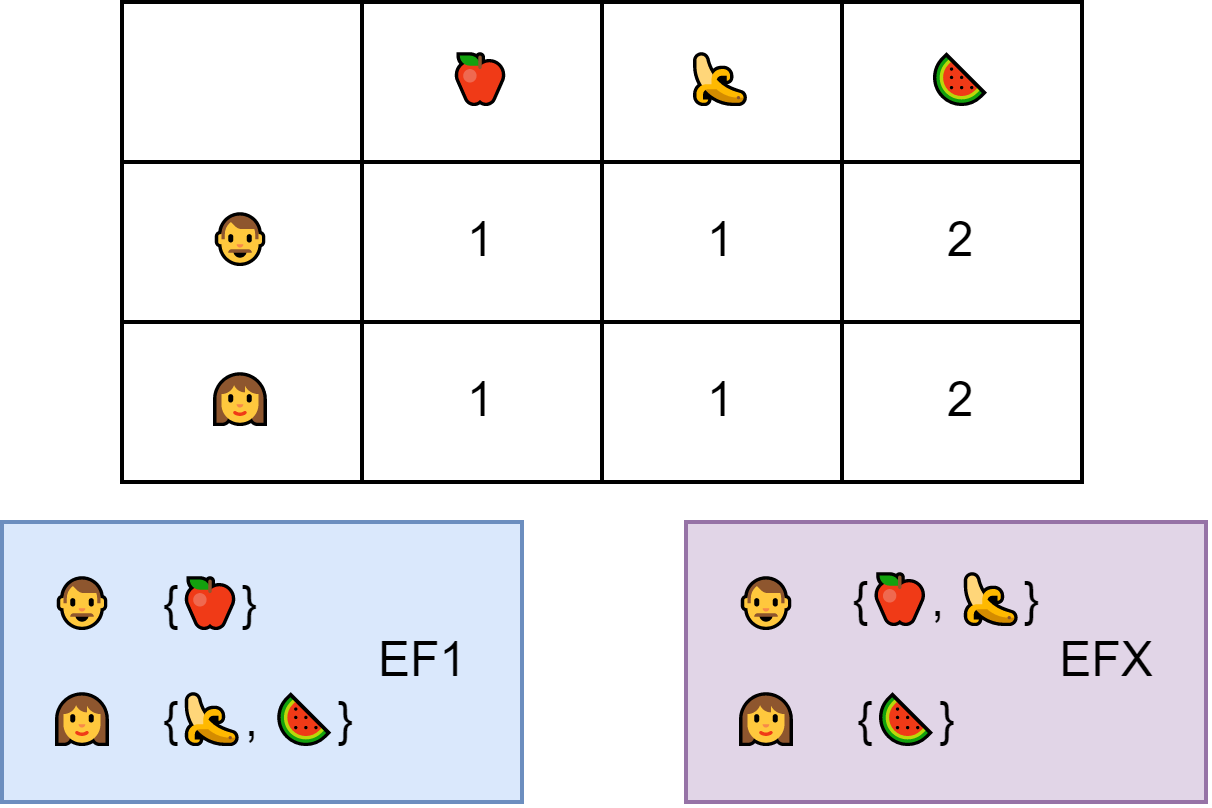
\includegraphics[width=0.5\textwidth]{image/EFX.png}
    \caption{Example of EF1 and EFX}
    \label{fig:example}
\end{figure}


\section{Core Ideas} \label{sec:core}

\subsection{Overview of EFX Allocation Algorithm}

In this section, we provide a formal and academic overview of the main ideas used to find our EFX (Envy-Free up to any number of goods) allocation. We begin by presenting the algorithm of Lipton et al. \cite{10.1145/988772.988792}, which is utilized to find an EF1 (Envy-Free with one good) allocation. Our approach extends this algorithm to achieve an EFX allocation, ensuring that no agent envies others even when multiple goods are involved.

\subsubsection{Algorithm for EF1 Allocation}

Lipton et al.'s algorithm \cite{10.1145/988772.988792} centers around the notion of an envy-graph, where each vertex represents an agent, and an edge $(i, j)$ exists if agent $i$ envies agent $j$. A crucial property of the envy-graph is that it forms a Directed Acyclic Graph (DAG). The absence of cycles in the envy-graph implies that no agent's envy can lead to a "chain reaction" of envy among other agents.

To ensure an EF1 allocation, the algorithm operates in rounds. At the beginning of each round, the envy-graph is checked for cycles. If a cycle is found, bundles are exchanged among the agents within the cycle to increase their individual valuations. This exchange eliminates cycles, and the process is repeated until no cycles remain in the envy-graph.

\subsubsection{Extension to EFX Allocation}

Our goal is to extend the algorithm to achieve an EFX allocation, where envy is eliminated not just for single goods, but for any number of goods. To maintain the EF1 property while incorporating multiple goods, we perform an allocation in each round, ensuring that the allocation remains EF1.

During each round, we identify an unenvied agent $s$, who becomes a source vertex in the envy-graph. We then allocate an unallocated good $g$ to agent $s$. As no other agent envies $s$ due to the unallocated good $g$, the new allocation remains EF1.

By repeating this process, we create an EFX allocation in which no agent envies others, regardless of the number of goods involved. This is achieved by systematically identifying unenvied agents and allocating unallocated goods to them, maintaining the EF1 property throughout the process.

\subsubsection{Conclusion}

In conclusion, we have presented a formal overview of the main ideas behind our EFX allocation algorithm, building upon the EF1 algorithm proposed by Lipton et al. \cite{10.1145/988772.988792}. By extending their approach to handle multiple goods, we achieve an EFX allocation, eliminating envy among agents for any number of goods. Our algorithm's effectiveness lies in its ability to identify unenvied agents and allocate goods to maintain the EF1 property, leading to a fair and envy-free allocation.

\subsection{The Reallocation Operation}

In this section, we elucidate a fundamental distinction between an EF1 allocation and an EFX allocation. The algorithm proposed by Lipton et al.~\cite{10.1145/988772.988792} reveals that given an EF1 allocation on a set $M_0$ of goods, it is possible to determine an EF1 allocation on $M_0 \cup M_1$, where $M_1 \subseteq M \setminus M_0$, by incrementally incorporating goods from $M_1$ into the existing bundles while cleverly adjusting ownership, if necessary. Essentially, this approach avoids the need for cutting or merging bundles during the EF1 allocation process, as the unallocated goods can be seamlessly appended to the current bundles.

However, the same strategy does not hold true for EFX allocations. To illustrate this point, consider the following example involving three agents with additive valuations and four goods \(a\), \(b\), \(c\), and \(d\).

\begin{figure}[htbp]
    \centering
    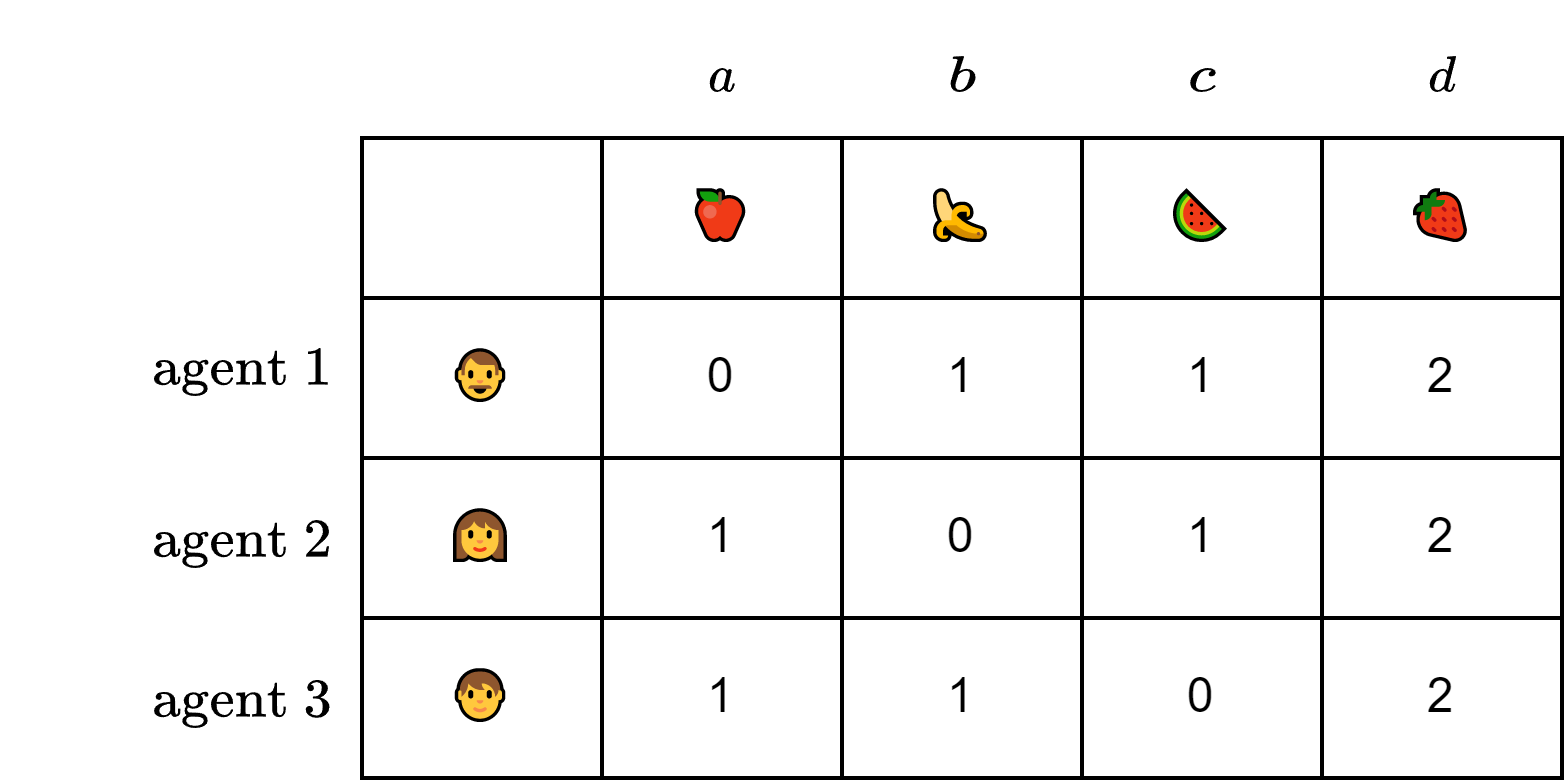
\includegraphics[width=0.5\textwidth]{image/EFX2.png}
    \caption{Illustration of three agents with additive valuations and four goods.}
    \label{fig:example3}
\end{figure}

For an EFX allocation of the first three goods, each of the three agents must receive exactly one good from the set \(a\), \(b\), and \(c\). However, in an EFX allocation involving all four goods, one agent (e.g., agent 1) must be allocated the singleton set \(\{d\}\), agent 2 receives \(\{a\}\), and agent 3 is assigned \(\{b, c\}\). This scenario necessitates cutting and merging bundles, which diverges from the straightforward approach used in EF1 allocations. When dealing with multiple agents, each having their unique valuations, identifying the appropriate cut-and-merge operations becomes the challenging aspect. In this section, we propose our global reallocation operation as a solution to this complexity.


\subsection{Improving Social Welfare}

In this section, we aim to improve the social welfare of an existing EFX allocation \(X = \langle X_1, \ldots, X_n\rangle \) on a given subset \(M_0 \subset M\). Our goal is to add a new good \(g \in M \setminus M_0\) to the allocation. However, we cannot guarantee that the resulting allocation on \(M_0 \cup \{g\}\) will still be EFX. Instead, we ensure that either of the following cases occurs:

(i) We obtain an EFX allocation \(X' = \langle X'_{1}, \ldots, X'_{n}\rangle\) on a subset of \(M_0 \cup \{g\}\) that satisfies \(v_i(X'_{i}) \geq v_i(X_i)\) for all agents \(i\), and for at least one agent \(j\), we have \(v_j(X'_{j}) > v_j(X_j)\). Consequently, the social welfare strictly improves, i.e., \(\sum_{i \in [n]} v_i(X'_{i}) > \sum_{i \in [n]} v_i(X_i)\).

(ii) We have an EFX allocation on \(M_0 \cup \{g\}\), and the social welfare does not decrease.

Thus, at each step of our algorithm, we either increase the social welfare or increase the number of allocated goods without reducing the social welfare. This ensures continuous progress in our approach, similar to the technique used by Plaut and Roughgarden~\cite{DBLP:journals/corr/PlautR17} to guarantee the existence of $1/2$-EFX in the case of agents having subadditive valuations. We now present an outline of how we achieve one of the cases (i) or (ii) in the allocation process.

For clarity, let's assume that the envy-graph corresponding to our initial EFX allocation \(X\) has a single source \(s\). To incorporate the new good \(g\), we add it to \(s\)'s bundle. If none of the other agents envy \(s\) after this addition, we obtain an EFX allocation on \(M_0 \cup \{g\}\), making this an easy case. In such instances, we "decycle" the envy-graph, if any cycles are created during the process, and proceed further. It is noteworthy that exchanging bundles along a cycle in the envy-graph results in an increase in the overall social welfare.

\subsection{Most Envious Agent}

In this section, we address the problem of envy among agents during the allocation of goods. Consider a scenario where one or more agents may envy another agent, denoted as $s$, up to any good after a particular good, denoted as $g$, is allocated to $s$. To resolve such envy, we introduce the concept of the "most envious agent."

Let $i$ be an agent who envies agent $s$ up to any good, meaning that there exists a subset $S' \subset X_s \cup \{g\}$ such that $v_i(X_i) < v_i(S')$. We define $S_i$ as an inclusion-wise minimal subset of $X_s \cup \{g\}$ for which $v_i(X_i) < v_i(S_i)$, with ties broken arbitrarily. Furthermore, for any subset $T \subset S_i$, it holds that $v_i(X_i) \geq v_i(T)$.

An agent $i$ will be termed the most envious agent of $X_s \cup \{g\}$ if $v_i(X_i) < v_i(S_i)$ for some $S_i \subset X_s \cup \{g\}$, and no strict subset of $S_i$ is envied by any other agent. In other words, $i$ is the most envious agent if no other agent envies any proper subset of $S_i$.

Let $t$ be the most envious agent of $X_s \cup \{g\}$. We observe that no agent envies the allocation $S_t$ up to any good. If an agent were to envy $S_t$ up to any good, it would contradict the fact that $S_t$ is an "inclusion-wise minimal envied set," meaning that no proper subset of $S_t$ is envied by any other agent. Given that the only source of envy is $s$, there exists a path $s \rightarrow i_1 \rightarrow \ldots \rightarrow i_{k-1} \rightarrow t$ in the envy graph.

To eliminate envy, we perform a leftwise shift of bundles along this path. Specifically, we allocate agent $s$ the bundle of agent $i_1$, and for $1 \leq r \leq k - 1$, agent $i_r$ receives the bundle of agent $i_{r+1}$ (where $i_k = t$). Finally, agent $t$ is allocated the bundle $S_t$. Any goods in $X_s \cup \{g\} \setminus S_t$ are returned to the pool of unallocated goods.

The result of this redistribution is that every agent in the path $s \rightarrow i_1 \rightarrow \ldots \rightarrow i_{k-1} \rightarrow t$ is strictly better off than in the initial allocation $X$, and no other agent is worse off. Moreover, by the definition of $S_t$, there is no agent who envies any other agent up to any good in the new allocation. As a result, we achieve a desirable envy-free exchange (EFX) allocation denoted as $X_0$.

This technique can be adapted for scenarios with multiple sources, provided there are enough unallocated goods. Specifically, the number of unallocated goods must be at least the number of sources in the envy graph. Further details on this adaptation are described in Section “Existence of an EFX-Allocation with Bounded Charity”.\footnote{We don't discuss the case where the number of unallocated goods is less than the number of sources in the envy graph. In such instances, we can use the algorithm by Plaut and Roughgarden~\cite{DBLP:journals/corr/PlautR17} to obtain a $1/2$-EFX allocation.}

It is worth noting that this approach differs from other EFX algorithms proposed by Plaut and Roughgarden~\cite{DBLP:journals/corr/PlautR17} and Caragiannis et al.~\cite{DBLP:journals/corr/abs-1902-04319}. The $1/2$-EFX algorithm by Plaut and Roughgarden either merges the new good $g$ with an existing bundle or allocates the singleton set $\{g\}$ to an agent. On the other hand, the EFX-with-charity algorithm by Caragiannis et al. takes an allocation of maximum Nash social welfare as input and then permanently removes some goods from the instance. Our notion of the "most envious agent" offers a novel way to break up a bundle, thereby preserving envy-freeness up to any good, which contributes to the innovation of our work.

\subsection{Other Results}

% Regarding our result with approximate MMS guarantee, if the number of unallocated goods in our EFX allocation is large, then the number of sources also has to be large: these are unenvied agents. Moreover, no agent envies the set of unallocated goods. Suppose for now that $|P| = n - 1$. This means every agent is a source. So no agent envies the bundle of any other agent and also the set of unallocated goods. Thus for each agent $i$, we have:
% \[
% v_i(X_i) \geq \frac{v_i(M)}{n + 1} \geq \left(1 + \frac{1}{n}\right)^{-1} \cdot \frac{v_i(M)}{n} \geq \left(1 - \frac{1}{n}\right) \cdot \text{MMS}_i(n, M),
% \]
% where the constraint that $\frac{v_i(M)}{n} \geq \text{MMS}_i(n, M)$ holds for additive valuations. We show our result for approximate-MMS allocation and our improved bound for approximate-GMMS allocation in Section “Guarantees on Other Notions of Fairness”.

In this section, we discuss additional findings concerning our EFX allocation with an approximate Maximin Share (MMS) guarantee. We observe that when the number of unallocated goods in our allocation is large, a corresponding increase in the number of sources (unenvied agents) is necessary. Furthermore, in our proposed EFX allocation, no agent envies the set of unallocated goods.

Let us consider the case where $|P| = n - 1$, implying that every agent is a source. As a result, no agent envies the bundle of any other agent, including the set of unallocated goods. For each agent $i$, the following inequality holds:

\[
v_i(X_i) \geq \frac{v_i(M)}{n + 1} \geq \left(1 + \frac{1}{n}\right)^{-1} \cdot \frac{v_i(M)}{n} \geq \left(1 - \frac{1}{n}\right) \cdot \text{MMS}_i(n, M),
\]

where the constraint $\frac{v_i(M)}{n} \geq \text{MMS}_i(n, M)$ is valid for additive valuations. We present our result for approximate-MMS allocation and an improved bound for approximate-Groupwise Maximin Share (GMMS) allocation in the section titled “Guarantees on Other Notions of Fairness”.


\section{Acknowledgement} \label{sec:ack}

I would like to express my sincere gratitude to my teacher, Professor Zhengyang Liu, for his exceptional dedication and expertise in teaching. His care, warmth, and continuous efforts to improve his teaching skills have greatly contributed to my academic growth. Throughout this course on Algorithmic Game Theory, I have gained a preliminary understanding of the subject and have made significant progress while completing the required report.

The reason I chose to write about the paper “A Little Charity Guarantees Almost Envy-Freeness” is that I was intrigued by the title and wanted to learn more about the topic. Moreover, I believe that maybe most of us don't know much about the charity, and I hope that through this paper, we can learn that such charity can lead to a better allocation of resources. With envy-freeness being a well-studied problem in the field of algorithmic game theory, I was curious to learn more about the topic and how it relates to the real world. I was also interested in the mathematical proofs and theorems presented in the paper and wanted to challenge myself to understand them (actually the mathematical proofs is really hard).

As I delved deeper into the article, I was pleasantly surprised to find that with concerted effort and proper application of reading techniques, I could effectively comprehend a lengthy academic paper filled with mathematical theorems. My past struggles of reading such papers from beginning to end with limited understanding have been replaced with the ability to grasp the meaning of the entire proof through its elegant derivation. Moreover, I have developed an intuitive understanding of the theorems and am impressed by their practical implications when applied to real-world scenarios.

In all of my assignments, I have endeavored to showcase my sincerity and dedication to the subject matter. I approached the proofs in my homework with rigor, ensuring their accuracy and validity. Similarly, in narrating the contents of the paper in my report, I have maintained a clear and logical presentation while incorporating my own understanding.

As an undergraduate student, I recognize the privilege of being a part of this learning experience and the opportunities it has provided for personal and academic growth. With deep appreciation, I humbly request that my efforts be acknowledged with a grade of 95+. However, regardless of the final grade, I am truly thankful for the invaluable knowledge and skills I have acquired during this course.

Thank you once again for your guidance and support.



\bibliographystyle{plain}
\bibliography{bibliography.bib}


% appendix
\appendix
\section{Appendix}

The Original tex code is in the \texttt{final.tex}.





\end{document}